\documentclass[12pt]{article}
\usepackage[utf8]{inputenc}
\usepackage{geometry}
\geometry{letterpaper, margin=0.25in}
\usepackage{graphicx} 
\usepackage{parskip}
\usepackage{booktabs}
\usepackage{array} 
\usepackage{paralist} 
\usepackage{verbatim}
\usepackage{subfig}
\usepackage{fancyhdr}
\usepackage{sectsty}
\usepackage{multicol}
\usepackage[shortlabels]{enumitem}

\pagestyle{fancy}
\renewcommand{\headrulewidth}{0pt} 
\lhead{}\chead{}\rhead{}
\lfoot{}\cfoot{\thepage}\rfoot{}

%%% ToC (table of contents) APPEARANCE
\usepackage[nottoc,notlof,notlot]{tocbibind} 
\usepackage[titles,subfigure]{tocloft}
\renewcommand{\cftsecfont}{\rmfamily\mdseries\upshape}
\renewcommand{\cftsecpagefont}{\rmfamily\mdseries\upshape} %

\usepackage{amsmath}
\usepackage{amssymb}
\usepackage{mathtools}
\usepackage{empheq}
\usepackage{xcolor}
\usepackage{bbm}
\usepackage{tikz}
\usepackage{pgfplots}
\usepackage{tikz-cd}
\pgfplotsset{compat=1.18}
\usetikzlibrary{intersections, decorations.markings}
\tikzset{
    marking along/.style n args={2}{
        decoration={
                markings, 
                mark=at position #1 with {\arrow{#2}}
        },
        postaction={decorate}
        },
    marking along/.default={0.5}{>}
}

\newcommand{\ans}[1]{\boxed{\text{#1}}}
\newcommand{\vecs}[1]{\langle #1\rangle}
\renewcommand{\hat}[1]{\widehat{#1}}

\renewcommand{\P}{\mathbb{P}}
\newcommand{\R}{\mathbb{R}}
\newcommand{\E}{\mathbb{E}}
\newcommand{\Z}{\mathbb{Z}}
\newcommand{\N}{\mathbb{N}}
\newcommand{\Q}{\mathbb{Q}}
\newcommand{\C}{\mathbb{C}}

\newcommand{\ind}{\mathbbm{1}}
\newcommand{\qed}{\quad \blacksquare}

\newcommand{\brak}[1]{\left\langle #1 \right\rangle}
\newcommand{\bra}[1]{\left\langle #1 \right\vert}
\newcommand{\ket}[1]{\left\vert #1 \right\rangle}

\newcommand{\abs}[1]{\left\vert #1 \right\vert}
\newcommand{\mfX}{\mathfrak{X}}
\newcommand{\ep}{\varepsilon}

\newcommand{\Ec}{\mathcal{E}}
\newcommand{\A}{\mathcal{A}}
\newcommand{\F}{\mathcal{F}}
\newcommand{\Cc}{\mathcal{C}}
\newcommand{\B}{\mathcal{B}}
\newcommand{\M}{\mathcal{M}}
\newcommand{\X}{\chi}
\renewcommand{\L}{\mathcal{L}}

\newcommand{\sub}{\subseteq}
\newcommand{\st}{\text{ s.t. }}
\newcommand{\card}{\text{card }}
\renewcommand{\div}{\vspace*{10pt}\hrule\vspace*{10pt}}
\newcommand{\surj}{\twoheadrightarrow}
\newcommand{\inj}{\hookrightarrow}
\newcommand{\biject}{\hookrightarrow \hspace{-8pt} \rightarrow}
\renewcommand{\bar}[1]{\overline{#1}}
\newcommand{\overcirc}[1]{\overset{\circ}{#1}}
\newcommand{\diam}{\text{diam }}

\renewcommand{\Re}{\text{Re}\,}
\renewcommand{\Im}{\text{Im}\,}
\newcommand{\sign}{\text{sign}\,}

\newcommand*{\tbf}[1]{\ifmmode\mathbf{#1}\else\textbf{#1}\fi}

\usepackage{tcolorbox}
\tcbuselibrary{breakable, skins}
\tcbset{enhanced}
\newenvironment*{tbox}[2][gray]{
    \begin{tcolorbox}[
        parbox=false,
        colback=#1!5!white,
        colframe=#1!75!black,
        breakable,
        title={#2}
    ]}
    {\end{tcolorbox}}

\newenvironment*{exercise}[1][red]{
    \begin{tcolorbox}[
        parbox=false,
        colback=#1!5!white,
        colframe=#1!75!black,
        breakable
    ]}
    {\end{tcolorbox}}

\newenvironment*{proof}[1][blue]{
\begin{tcolorbox}[
    parbox=false,
    colback=#1!5!white,
    colframe=#1!75!black,
    breakable
]}
{\end{tcolorbox}}

\newenvironment{proposition}[1][gray]{
\begin{tcolorbox}[
    parbox=false,
    colback=#1!5!white,
    colframe=#1!75!black,
    breakable
]}
{\end{tcolorbox}}

\title{APMA 1360: Midterm 1 Review}
\author{}
\date{}

\begin{document}
\begin{multicols}{2}
    \begin{proposition}
        \textbf{Theorem (Existence and Uniqueness):} Consider $\dot u = f(u)$ with $u(0) = u_0$. Assume $u \in \R^2$ and $f \in C^1$. Then there exists a unique solution to the ODE on some interval around $t=0$.
    \end{proposition}

    \tbf{Equilibrium:} If $\dot u = f(u) = 0$ at $u_*$, then $u_*$ is an \emph{equilibrium}.
    \begin{itemize}
        \item If $f'(u_*) < 0$, then $u_*$ is \emph{stable}
        \item If $f'(u_*) > 0$, then $u_*$ is \emph{unstable}
    \end{itemize}

    \tbf{Phase diagrams:}
    \begin{enumerate}
        \item Plot $f$
        \item Zeros of $f$ are equilibrium points
        \item If $f$ changes from positive to negative at the equilibrium, it is stable
        \item If $f$ changes from negative to positive at the equilibrium, it is unstable
        \item Otherwise, it is a saddle
    \end{enumerate}

    \begin{proposition}
        \textbf{Implicit Function Theorem:} Let $f: \R^2 \to \R$ be a $C^k$ ($k \geq 1$) function. Assume $f(x_*, y_*) = 0$.

        Then:
        \begin{enumerate}
            \item If $f_x(x_*, y_*) \neq 0$, then $\exists ! g: B_{\ep}(y_*) \to \R$ with $x_* = g(y_*)$ and $g \in C^k$ such that $f(x, y) = 0 \iff x = g(y)$ for $(x, y) \in B_{\ep}(x_*) \times B_{\ep}(y_*)$
            \item If $f_y(x_*, u_) \neq 0$, then $\exists ! h: B_{\ep}(x_*) \to \R$ with $y_* = h(x_*)$ and $h \in C^k$ such that $f(x, y) = 0 \iff y = g(x)$ for $(x, y) \in B_{\ep}(x_*) \times B_{\ep}(y_*)$
        \end{enumerate}

    \end{proposition}

    \tbf{Example:} Find all zeros of $f(x, y) = y + y^2 e^x + (\sin x)^2 - xy$ near $(0, 0)$.
    \begin{enumerate}
        \item Check conditions:
              \begin{itemize}
                  \item $f \in C^{\infty}$
                  \item $f(0, 0) = 0$
                  \item $f_x(0, 0) = (0)^2 (1) + 2(0)(1) - (0) = 0$
                  \item $f_y(0, 0) = 1 + 2(0)(1) - (0) \neq 0$
              \end{itemize}
        \item Apply IFT to get $f(x, y) = 0$ iff $x = g(y)$ with $g(0) = 0$
        \item Taylor expand $f$:
              \[g(x) = g(0) + xg'(0) + O(x^2) = xg'(0) + O(x^2) = O(x)\]
    \end{enumerate}

    \tbf{Hyperbolic Equilibrium:} If $f(u_*, \mu_*) = 0$ and $f_u(u_*, \mu_*) \neq 0$, we say $(u_*, \mu_*)$ is \emph{hyperbolic}

    \subsection{Catelogue of bifurcations:}

    \tbf{Saddle-node:} $\dot u = \mu - u^2$
    \[\begin{cases}
            f(u_*, \mu_*) = 0          \\
            f_u(u_*, \mu_*) = 0        \\
            f_{\mu}(u_*, \mu_*) \neq 0 \\
            f_{uu}(u_*, \mu_*) \neq 0
        \end{cases}\]

    \tbf{Transcritical:} $\dot u = u(u - \mu)$.
    \[\begin{cases}
            f(0, \mu) = 0         \\
            f_u(0, 0) =0          \\
            f_{u\mu}(0, 0) \neq 0 \\
            f_{uu}(0, 0) \neq 0
        \end{cases}\]

    \tbf{Pitchfork:} $\dot u = \mu u - u^3$
    \[\begin{cases}
            f(-u, \mu) = -f(u, \mu) \\
            f_u(0, 0) = 0           \\
            f_{u\mu}(0, 0) \neq 0   \\
            f_{uuu}(0, 0) \neq 0
        \end{cases}\]

    Which has two forms:
    \begin{center}
        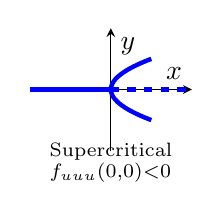
\begin{tikzpicture}
            \begin{axis}[
                    width=0.3\textwidth,
                    axis lines=middle,
                    no markers,
                    xtick=\empty,
                    ytick=\empty,
                    clip=false,
                    xlabel={$x$},
                    ylabel={$y$},
                    domain=-1:1,
                    ymin=-2, ymax=2,
                    xmin= -2, xmax=2,
                    view = {0}{90}
                ]
                \addplot[ultra thick, blue, domain=-2:0] {0};
                \addplot[ultra thick, blue, dashed, domain=0:2] {0};
                \addplot[ultra thick, blue, domain=-1:1] ({x^2}, {x});

                \node at (axis description cs: 0.5, -0.1) {$\begin{subarray}{align*}
                            \text{Supercritical} \\
                            f_{uuu}(0, 0) < 0
                        \end{subarray}$};
            \end{axis}
        \end{tikzpicture}

        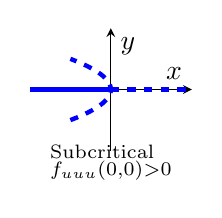
\begin{tikzpicture}
            \begin{axis}[
                    width=0.3\textwidth,
                    axis lines=middle,
                    no markers,
                    xtick=\empty,
                    ytick=\empty,
                    clip=false,
                    xlabel={$x$},
                    ylabel={$y$},
                    domain=-1:1,
                    ymin=-2, ymax=2,
                    xmin= -2, xmax=2,
                    view = {0}{90}
                ]
                \addplot[ultra thick, blue, domain=-2:0] {0};
                \addplot[ultra thick, blue, dashed, domain=0:2] {0};
                \addplot[ultra thick, blue, dashed, domain=-1:1] ({-x^2}, {x});

                \node at (axis description cs: 0.5, -0.1) {$\begin{subarray}{align*}
                            \text{Subcritical} \\
                            f_{uuu}(0, 0) > 0
                        \end{subarray}$};
            \end{axis}
        \end{tikzpicture}
    \end{center}

    \subsection{Multidimensional Systems}
    For $\dot u = f(u)$ with $u \in \R^n$ and $f: \R^n \to \R^n$, we have two different methods for solving:
    \begin{enumerate}
        \item Find the eigenvalues of the Jacobian $Df(u_i)$ to determine stability for each equilibrium $u_i$
        \item Plot nullclines and examine what the gradient does at each region of the phase plane. Notice the gradient $\nabla h$ is always perpendicular to the nullcline and pointing in the firection of increasing $h$.
    \end{enumerate}

    \tbf{Nullcline:} $\{(x, y): \dot x = 0\}$ or $\{(x, y): \dot y = 0\}$. Where the nullclines intersect are the equilibrium points.

\end{multicols}
\pagebreak

\section{Practice Problems}

\tbf{1.} Consider the system $\dot x = x(r - 2 -x)$
\begin{enumerate}[(a)]
    \item Determine all fixed points

          \color{blue}
          $x = 0$ and $x = r - 2$.
          \color{black}

    \item Classify the stability as a function of $r$
          \color{blue}
          $f(x) = x(r - 2 - x)$. $f'(x) = r - 2 - 2x$ so $f'(0) = r - 2$ and $f'(r - 2) = -r + 2$. Thus, $x = 0$ is stable for $r < 2$ and $x = r - 2$ is stable for $r > 2$.
          \color{black}

    \item Sketch all qualitatively different phase portraits

          \begin{center}
              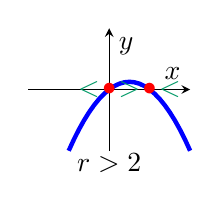
\begin{tikzpicture}
                  \begin{axis}[
                          width=0.3\textwidth,
                          axis lines=middle,
                          no markers,
                          xtick=\empty,
                          ytick=\empty,
                          clip=false,
                          xlabel={$x$},
                          ylabel={$y$},
                          domain=-2:2,
                          ymin=-2, ymax=2,
                          xmin= -2, xmax=2,
                          view = {0}{90}
                      ]
                      \addplot[ultra thick, blue, domain=-1:2] {x*(1-x)};
                      \node[red] at (0, 0) {$\bullet$};
                      \node[red] at (1, 0) {$\bullet$};

                      \node[teal!80!green] at (-0.5, 0) {$<$};
                      \node[teal!80!green] at (0.5, 0) {$>$};
                      \node[teal!80!green] at (1.5, 0) {$<$};

                      \node at (axis description cs: 0.5, -0.1) {$r > 2$};
                  \end{axis}
              \end{tikzpicture}
              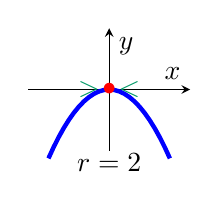
\begin{tikzpicture}
                  \begin{axis}[
                          width=0.3\textwidth,
                          axis lines=middle,
                          no markers,
                          xtick=\empty,
                          ytick=\empty,
                          clip=false,
                          xlabel={$x$},
                          ylabel={$y$},
                          domain=-1.5:1.5,
                          ymin=-2, ymax=2,
                          xmin= -2, xmax=2,
                          view = {0}{90}
                      ]
                      \addplot[ultra thick, blue] {-x^2};
                      \node[red] at (0, 0) {$\bullet$};

                      \node[teal!80!green] at (-0.5, 0) {$>$};
                      \node[teal!80!green] at (0.5, 0) {$<$};


                      \node at (axis description cs: 0.5, -0.1) {$r = 2$};
                  \end{axis}
              \end{tikzpicture}
              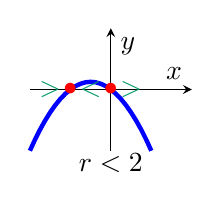
\begin{tikzpicture}
                  \begin{axis}[
                          width=0.3\textwidth,
                          axis lines=middle,
                          no markers,
                          xtick=\empty,
                          ytick=\empty,
                          clip=false,
                          xlabel={$x$},
                          ylabel={$y$},
                          domain=-2:2,
                          ymin=-2, ymax=2,
                          xmin= -2, xmax=2,
                          view = {0}{90}
                      ]
                      \addplot[ultra thick, blue, domain=-2:1] {x*(-1-x)};
                      \node[red] at (0, 0) {$\bullet$};
                      \node[red] at (-1, 0) {$\bullet$};

                      \node[teal!80!green] at (-1.5, 0) {$>$};
                      \node[teal!80!green] at (-0.5, 0) {$<$};
                      \node[teal!80!green] at (0.5, 0) {$>$};

                      \node at (axis description cs: 0.5, -0.1) {$r < 2$};
                  \end{axis}
              \end{tikzpicture}
          \end{center}
    \item Sketch the bifurcation diagram and identify the type of bifurcation

          \begin{center}
              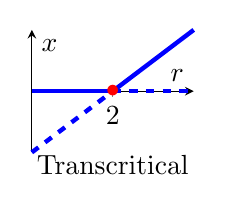
\begin{tikzpicture}
                  \begin{axis}[
                          width=0.3\textwidth,
                          axis lines=middle,
                          no markers,
                          xtick={2},
                          ytick=\empty,
                          clip=false,
                          xlabel={$r$},
                          ylabel={$x$},
                          domain=-2:2,
                          ymin=-2, ymax=2,
                          xmin= 0, xmax=4,
                          view = {0}{90}
                      ]
                      \addplot[ultra thick, blue, domain=0:2] {0};
                      \addplot[ultra thick, blue, dashed, domain=2:4] {0};

                      \addplot[ultra thick, blue, dashed, domain=0:2] {x-2};
                      \addplot[ultra thick, blue, domain=2:4] {x-2};

                      \node at (axis description cs: 0.5, -0.1) {Transcritical};

                      \node[red] at (2, 0) {$\bullet$};

                  \end{axis}
              \end{tikzpicture}
          \end{center}
\end{enumerate}


\tbf{2.} Make a phase portrait and classify all equilibria of the following system
\[\begin{cases}
        \dot x = x(3 - x) - 2xy \\
        \dot y = y(2- y) - xy
    \end{cases}\]

\color{blue}

We have Jacobian,
\[J(x, y) = \begin{pmatrix}
        3- 2x - 2y & -2x        \\
        -y         & 2 - 2y - x
    \end{pmatrix}\]

and nullclines
\begin{align*}
    \{(x, y): \dot x = 0\} & = \{(0, y)\} \cup \{(3, y)\} \cup \{(x, \frac{3-x}{2})\} \\
    \{(x, y): \dot y = 0\} & = \{(x, 0)\} \cup \{(x, 2)\} \cup \{(2-y, y)\}
\end{align*}
which give us equilibria at $(0, 0)$, $(3, 0)$, $(0, 2)$, $(3, 2)$, and $(1, 1)$.

Hence, we know stabilities:
\color{red}
\begin{align*}
    J(0, 0) & = \begin{pmatrix}
                    3 & 0 \\
                    0 & 2
                \end{pmatrix} \implies \text{repeller}   \\
    J(3, 0) & = \begin{pmatrix}
                    -3 & -6 \\
                    0  & -3
                \end{pmatrix} \implies \text{attractor}  \\
    J(0, 2) & = \begin{pmatrix}
                    -1 & 0  \\
                    -2 & -2
                \end{pmatrix} \implies \text{attractor}  \\
    J(3, 2) & = \begin{pmatrix}
                    -7 & -6 \\
                    -2 & -5
                \end{pmatrix}  \implies \text{attractor} \\
    J(1, 1) & = \begin{pmatrix}
                    -1 & -2 \\
                    -1 & -1
                \end{pmatrix} \implies \text{saddle}
\end{align*}
\begin{center}
    \color{black}
    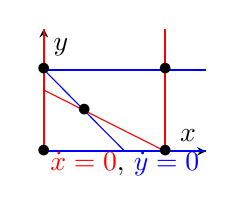
\begin{tikzpicture}
        \begin{axis}[
                width=0.3\textwidth,
                axis lines=middle,
                no markers,
                xtick=\empty,
                ytick=\empty,
                clip=false,
                xlabel={$x$},
                ylabel={$y$},
                domain=-2:2,
                ymin=0, ymax=3,
                xmin=0, xmax=4,
                view = {0}{90}
            ]
            \draw[red, thick] (0, 0) -- (0, 3);
            \draw[red, thick] (3, 0) -- (3, 3);

            \draw[blue, thick] (0, 0) -- (4, 0);
            \draw[blue, thick] (0, 2) -- (4, 2);

            \addplot[red, domain=0:3] {(3-x)/2};
            \addplot[blue, domain=0:2] {2-x};

            \node at (0, 0) {$\bullet$};
            \node at (3, 0) {$\bullet$};
            \node at (0, 2) {$\bullet$};
            \node at (3, 2) {$\bullet$};
            \node at (1, 1) {$\bullet$};


            \node at (axis description cs: 0.5, -0.1) {\textcolor{red}{$\dot x = 0$}, \textcolor{blue}{$\dot y = 0$}};

            %\draw[marking along] (0, 0) -- (3, 0);
            %\draw[marking along] (0, 0) -- (0, 2);
            %\draw[marking along] (0, 0) -- (1, 1);
            %
            %\draw[marking along] (1, 1) -- (3, 0);
            %\draw[marking along] (1, 1) -- (0, 2);
            %\draw[marking along] (1, 1) -- (3, 2);
        \end{axis}
    \end{tikzpicture}
\end{center}
\color{black}


\tbf{3.} Which of the following functions can we apply IFT at $(x, y) = (0, 0)$ and what does IFT give us?
\begin{enumerate}[(a)]
    \item $y^2 + x^2 + e^x - 1 = 0$

          \color{blue}
          \begin{itemize}
              \item $f(0, 0) = 0$
              \item $f_x(0, 0) = 1 \neq 0$
              \item $f_y(0, 0) = 0$
          \end{itemize}
          Hence we can apply IFT to get $g \in C^{\infty}$ with $f(x, y) = 0 \iff x = g(y)$ around $(0, 0)$.
          \color{black}

          \begin{center}
              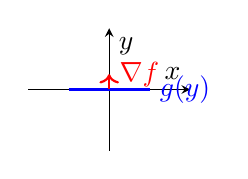
\begin{tikzpicture}
                  \begin{axis}[
                          width=0.3\textwidth,
                          axis lines=middle,
                          no markers,
                          xtick=\empty,
                          ytick=\empty,
                          clip=false,
                          xlabel={$x$},
                          ylabel={$y$},
                          domain=-2:2,
                          ymin=-2, ymax=2,
                          xmin= -2, xmax=2,
                          view = {0}{90}
                      ]
                      \draw[thick, blue] (-1, 0) -- (1, 0) node[right] {$g(y)$};
                      \draw[thick, red, ->] (0, 0) -- (0, 0.5) node[right] {$\nabla f$};

                  \end{axis}
              \end{tikzpicture}
          \end{center}

    \item $ye^x = 0$
          \color{blue}
          \begin{itemize}
              \item $f(0, 0) = 0$
              \item $f_x(0, 0) = 0$
              \item $f_y(0, 0) = 1 \neq 0$
          \end{itemize}
          so we can apply IFT to get $f(x, y) = 0\iff y = g(x)$.
          \color{black}

          \begin{center}
              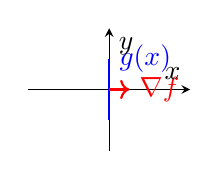
\begin{tikzpicture}
                  \begin{axis}[
                          width=0.3\textwidth,
                          axis lines=middle,
                          no markers,
                          xtick=\empty,
                          ytick=\empty,
                          clip=false,
                          xlabel={$x$},
                          ylabel={$y$},
                          domain=-2:2,
                          ymin=-2, ymax=2,
                          xmin= -2, xmax=2,
                          view = {0}{90}
                      ]
                      \draw[thick, blue] (0, -1) -- (0, 1) node[right] {$g(x)$};
                      \draw[thick, red, ->] (0, 0) -- (0.5, 0) node[right] {$\nabla f$};

                  \end{axis}
              \end{tikzpicture}
          \end{center}

    \item $\sin x + \sin y = 0$
          \color{blue}
          \begin{itemize}
              \item $f(0, 0) = 0$
              \item $f_x(0, 0) = 1$
              \item $f_y(0, 0) = 1$
          \end{itemize}
          so we can apply IFT in either variable.

          Further, $\nabla f = (1, 1)$ so we look something like

          \begin{center}
              \color{black}
              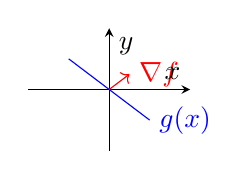
\begin{tikzpicture}
                  \begin{axis}[
                          width=0.3\textwidth,
                          axis lines=middle,
                          no markers,
                          xtick=\empty,
                          ytick=\empty,
                          clip=false,
                          xlabel={$x$},
                          ylabel={$y$},
                          domain=-2:2,
                          ymin=-2, ymax=2,
                          xmin= -2, xmax=2,
                          view = {0}{90}
                      ]

                      \draw[blue] (-1, 1) -- (1, -1) node[right] {$g(x)$};
                      \draw[red, ->] (0, 0) -- (0.5, 0.5) node[right] {$\nabla f$};

                  \end{axis}
              \end{tikzpicture}
          \end{center}
          \color{black}

\end{enumerate}
\end{document}